\section{Proposed Approach}
A single-stage Class AB power amplifier was designed to operate at a center frequency of 2.2\,GHz, targeting an output power of 30\,dBm for a drain efficiency of 30\% at the 1\,dB compression point, using the CGH40006S GaN HEMT transistor (MACOM) \cite{Macom}. The circuit was fabricated on a four-layer PCB manufactured by JLCPCB using the JLC04161H-7628 stackup, shown in Table~\ref{tab:pcb_stackup}, which provides a controlled 50\,$\Omega$ impedance for the transmission lines.

\begin{table}[b]
    \caption{PCB Stackup}
    \label{tab:pcb_stackup}
    \centering
    \renewcommand{\arraystretch}{1.1}
    \begin{tabular}{|l|c|c|}
        \hline
        \textbf{Layer} & \textbf{Relative Permittivity (Dk)} & \textbf{Thickness} \\
        \hline
        Top      & \cellcolor{coppercolor}Copper  & 0.035mm   \\ \hline
        Prepreg  & \cellcolor{dielectriccolor}4.4 & 0.21040mm \\ \hline
        Inner L2 & \cellcolor{coppercolor}Copper  & 0.0152mm  \\ \hline
        Core     & \cellcolor{dielectriccolor}4.6 & 1.065mm   \\ \hline
        Inner L3 & \cellcolor{coppercolor}Copper  & 0.0152mm  \\ \hline
        Prepreg  & \cellcolor{dielectriccolor}4.4 & 0.21040mm \\ \hline
        Bottom   & \cellcolor{coppercolor}Copper  & 0.035mm   \\
        \hline
    \end{tabular}
\end{table}

To allow post-fabrication tuning of the transmission lines, additional short traces were included close to other circuit traces throughout the PCB. These traces are unconnected and can be selectively incorporated to introduce stubs of variable length or to extend existing lines, enabling adjustment and further testing of the matching networks without requiring a new board revision. Fig.~\ref{fig:pcb} shows the fabricated PCB.

\begin{figure}[b]
    \centering
    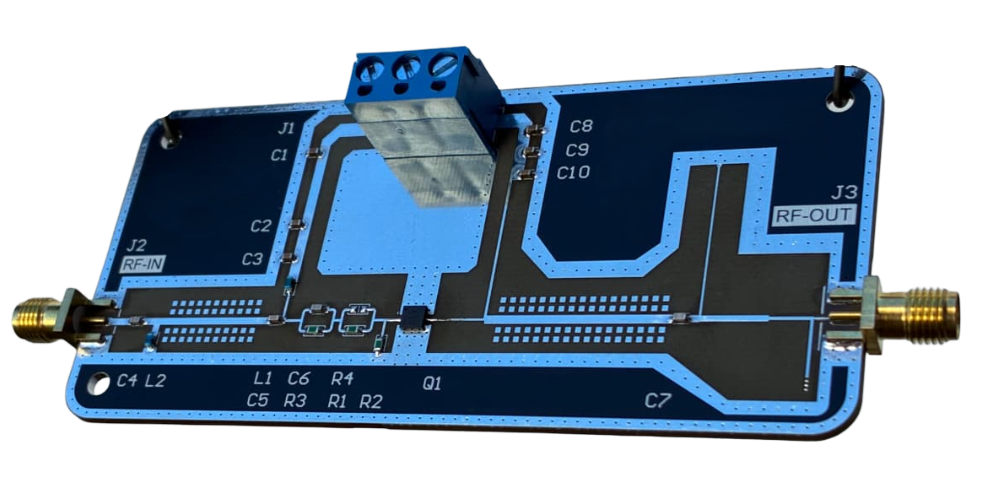
\includegraphics[width=\linewidth]{imgs/placa_sin_logos.png}
    \caption{Fabricated PCB of the proposed 2.2 GHz GaN power amplifier.}
    \label{fig:pcb}
\end{figure}

The overall architecture is shown in Fig.~\ref{fig:pa_diagram}. The input stage comprises a high-pass filter (HPF), a bias-tee, and a stability network, while the output stage consists of a bandpass filter (BPF) and a bias-tee. Both the input and output networks were designed to achieve impedance matching at the operating frequency, with the target impedances determined from load-pull simulation results.

\begin{figure*}[t]
    \centering
    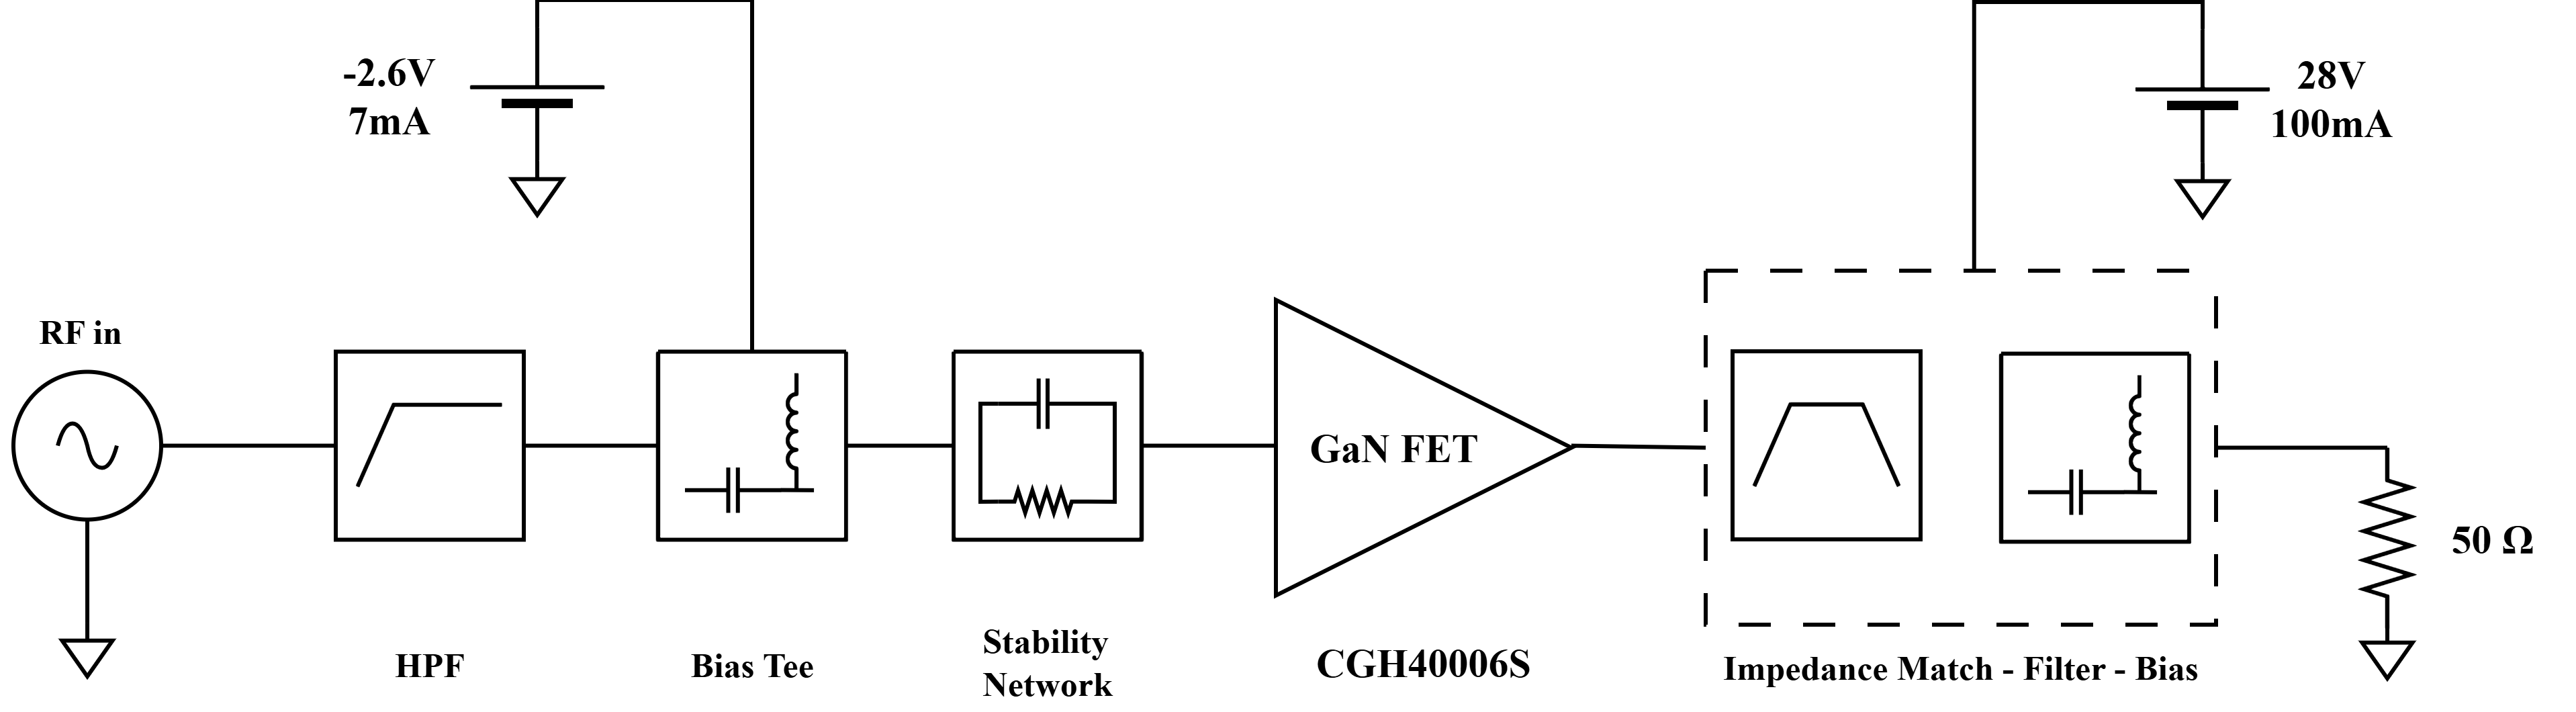
\includegraphics[width=\textwidth]{imgs/pa_block_diagram.png}
    \caption{Block diagram of the proposed power amplifier, including the input matching, biasing, stabilization, and output matching networks.}
    \label{fig:pa_diagram}
\end{figure*}

% =========================================================================== %
\subsection{Circuit Biasing}
Biasing is provided through a bias-tee at each port, consisting of an RF choke and a DC block capacitor. The RF choke presents a high impedance at the operating frequency, isolating the DC supply from the RF signal path, while the DC block capacitor prevents the DC bias from reaching the RF ports. Additional bypass capacitors were placed along the power supply rails to filter out supply noise. The bias point was set at a drain voltage $V_D = 28\,\text{V}$ and a gate voltage $V_G = -2.6\,\text{V}$, resulting in a drain current of $I_D = 100\,\text{mA}$ and a gate bias current of $7\,\text{mA}$, corresponding to Class AB operation.

% =========================================================================== %
\subsection{Simulation-assisted Design Methodology}
The circuit was simulated using a SPICE-based simulator with harmonic balance (HB) analysis. A transistor simulation model and passive component models, including transmission line models, were incorporated. Small-signal S-parameter simulations were used to evaluate the stability of the design over a broad frequency range (0.5–8\,GHz). Load-pull simulation was performed by sweeping input and load impedances under large-signal (HB analysis) conditions to map power-added efficiency (PAE), output power, and gain contours, enabling the selection of the optimal output termination impedance \cite{Cripps2006}.

% =========================================================================== %
\subsection{Load-Pull and Matching Networks}
Load-pull analysis sweeps the load impedance across the Smith chart under large-signal excitation, mapping figures of merit such as PAE, output power, and gain at each impedance point. The resulting contours enable the selection of the termination that best satisfies the target performance trade-off.

The output matching network was designed based on the results of load-pull simulation, which identified the optimal load impedance maximizing PAE at the target output power level. The input matching network was subsequently optimized to maximize power transfer and overall circuit performance. A point offering a favorable trade-off among PAE, gain, and output power was selected from the load-pull contours for an input power of 14 dBm, shown in Fig.~\ref{fig:loadpull_img}. The load-pull analysis determined an optimal load impedance of (24.1 + j52) $\Omega$.

% =========================================================================== %
\subsection{Stability Network}
The small-signal stability of an amplifier can be analyzed by studying the $\mu_{source}$ and $\mu_{load}$ parameters, derived from the S-parameters of the circuit. According to \cite{Edwards1992}, if either parameter exceeds unity for all frequencies, the circuit is unconditionally stable. This constitutes both a necessary and sufficient condition.

Unconditional stability was ensured across the 0.5–8 GHz frequency range by implementing a stabilization network at the transistor gate, consisting of a parallel RC circuit followed by a resistive voltage divider \cite{Bahl2009}. Additionally, a shunt resistor was included on the PCB as an optional post-fabrication tuning element to allow stability adjustments without requiring a board revision. To verify the network's effectiveness, both stability factors were extracted from simulated small-signal S-parameters. As illustrated in Fig.~\ref{fig:stability_img}, $\mu_{source}$ and $\mu_{load}$ exceed unity throughout the entire range, confirming the small-signal unconditional stability of the amplifier.

\begin{figure}
    \centering
    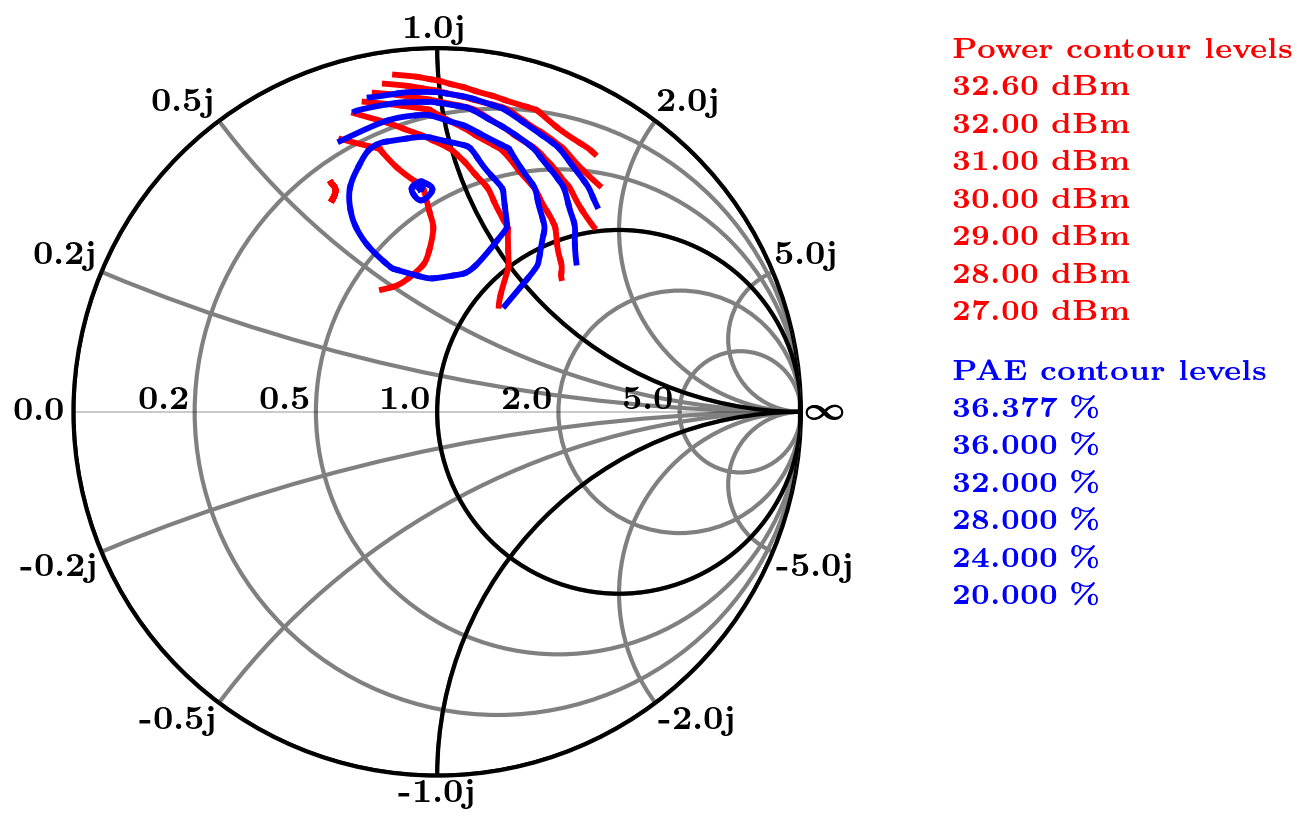
\includegraphics[width=0.48\textwidth]{imgs/load_pull_plot.png}
    \caption{Load-pull simulation contours: PAE (blue) and $P_{out}$ (red) on the Smith chart}
    \label{fig:loadpull_img}
    
    \vspace{0.5em}
    
    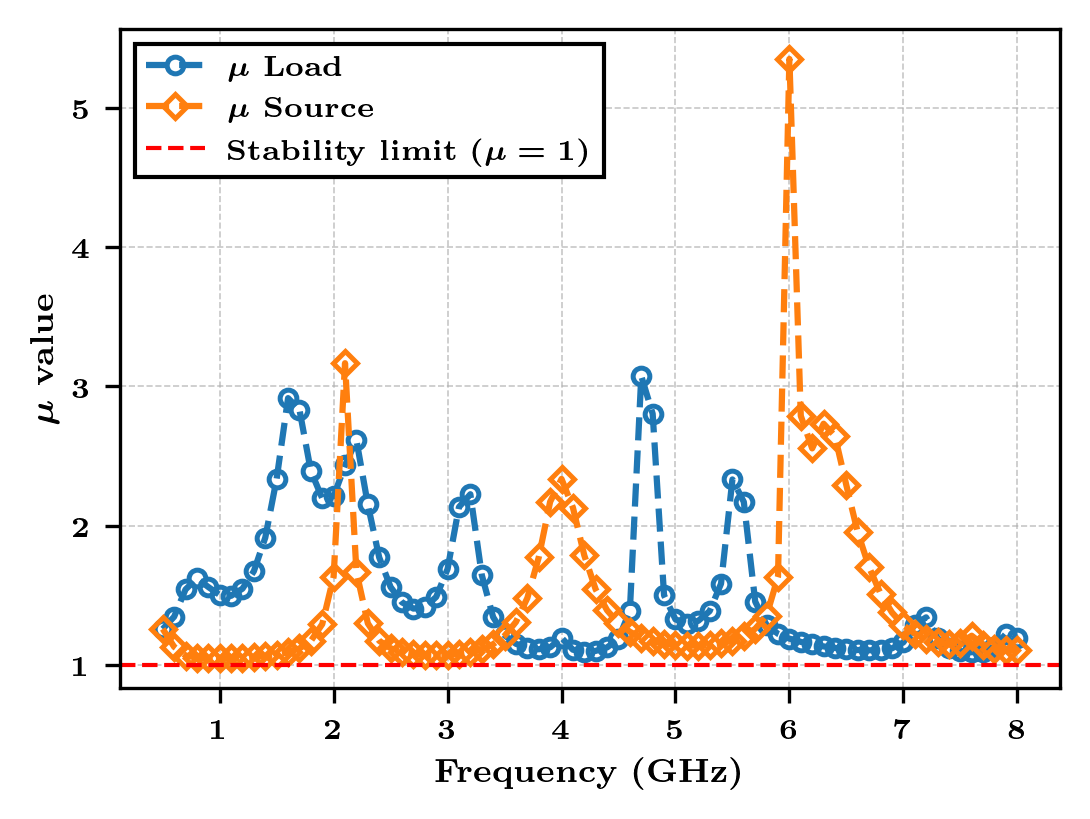
\includegraphics[width=0.48\textwidth]{imgs/stability_plot.png}
    \caption{Simulated source and load stability factors ($\mu$) as a function of frequency. The load stability factor (blue) and source stability factor (orange) remain above the unconditional stability threshold ($\mu=1$, red dashed line) across the whole frequency range, indicating stable operation.}
    \label{fig:stability_img}
\end{figure}

% =========================================================================== %
\subsection{Output Waveforms}
A 5th-order harmonic balance simulation was conducted to analyze the large-signal spectral response of the proposed design and evaluate the harmonic content at the output, providing insight into the nonlinear behavior of the amplifier under operating conditions. The input RF power was set to 14\,dBm into a 50\,$\Omega$ matched load. Fig.~\ref{fig:spectrum} shows the simulated output harmonic spectrum from the fundamental frequency up to the fifth harmonic.

\begin{figure}[t]
    \centering
    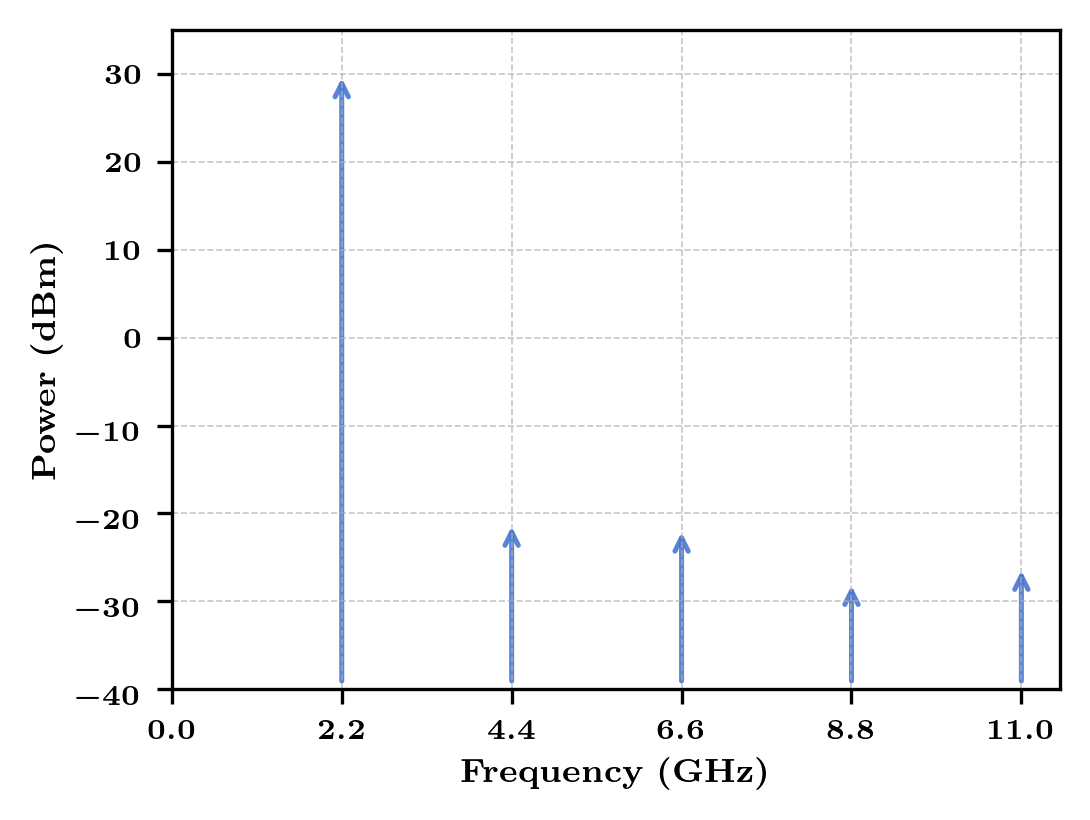
\includegraphics[width=\linewidth]{imgs/spectrum_plot.png}
    \caption{Harmonic balance simulation results showing the output power spectrum up to the fifth harmonic.}
    \label{fig:spectrum}
\end{figure}